\documentclass{article}
\usepackage{amsmath}
\usepackage{graphicx}
\usepackage{setspace}
\usepackage[affil-it]{authblk}
\usepackage[left=3cm, right=3cm, top=3cm, bottom=3cm]{geometry}
\usepackage{multicol}
\usepackage{listings}
\usepackage[linesnumbered,ruled,vlined]{algorithm2e}
\usepackage{algpseudocode,amsthm}
\usepackage{calrsfs}
\DeclareMathAlphabet{\pazocal}{OMS}{zplm}{m}{n}
% \setlength{\columnsep}{-4cm}
% \usepackage{tikz-qtree}
\usepackage[hidelinks]{hyperref}

\title{CS513: Graph}
\date{}
\author{Prateekshya Priyadarshini}
\affil{M.Tech CSE}
\setcounter{tocdepth}{3}
\begin{document}
\tableofcontents
\newpage
\pagenumbering{arabic}
\maketitle

\section{Introduction}
Graph is a data structure which can store relevant information in the nodes and connect them in a meaningful way with edges. These are the examples of some graphs.
\begin{center}
\includegraphics[scale=0.5]{graph1.png}
\includegraphics[scale=0.5]{graph2.png}
\end{center}
The left one is an undirected graph and the second one is a directed graph. We can also add weights to the edges. Those kind of graphs would be called \textbf{weighted graphs}. We can represent graphs using adjacency matrix or adjacency lists.\newline
For simplicity, here we do not store any information in the nodes. We simply number them from $0$ to $V-1$ where $V$ is the number of nodes.


\section{Related Work}
\subsection{Creating batch files or shell scripts}
Since the commands to generate a .png file from a .gv file are not straight forward for a beginner, this program generates batch file in windows and shell script in linux which contains all those commands. Every time a new tree is printed, these files get executed and the respective images get generated. For reference, the images won't be deleted or replaced till the program is being executed.
\subsection{Storing the entire execution process}
The entire execution process is stored in \textbf{output.txt}. This file can be referred to check what went wrong, which images refer to which trees etc.
\subsection{One combined print function}
There is only one function to generate the images of graphs which takes variable arguments as per the requirement.
\subsection{Use of unordered\_map}
Since there is a significant usage of unordered maps, follow the steps carefully if you're using Dev cpp for running the program.
\subsection{Variables to be fixed before execution}
There are a few variables those can be chaged before ecxecution. For now they are set to some default stable values. Those variables are listed in first four lines of \textbf{functions.h}. You can add more colours and set the noc values to the number of colours. Percentage ranges of dense, sparse or medium graphs can be changed as per requirement. There are two prime numbers being used to create custom hash values for edges. Try setting it to some higher values for avoiding key clashes.

This application works in two modes i.e. Build mode and Operations mode. The next two sections are dedicated for the description of these modes.

\section{Build Mode}
In build mode, we can create a new graph, add or remove edges from the existing graph and print the graph. We can also write a sequence of addition and removal of edges in a file and put it to execute those operations in bulk. This mode is present to make the execution flexible.
\subsection{void createGraph()}
This function asks us whether we want to give a manual input file or generate a random graph. For manual input file, we need to write a .txt file in the given format and write the file name in the console. If we choose random input file, it will further ask to choose the type of graph we want. We can choose one out of (sparse/medium/dense) graph. Alternatively we can give a percentage value. If we give the value as $15$, it will create $15\%$ of total possible edges in the graph. Self loops are not considered in total possible edges calculation, but it adds self loops in the graph. It generates an image for the newly created graph.
\subsection{void generateInput()}
It generates a random input file based on the parameters chosen.
\subsection{void executeModification()}
This function is meant for modifying an existing graph by adding or removing edges. If we try to perform a bulk modification, then int prints the new graph.
\subsection{void performBulkModification()}
This function takes a .txt file and performs all the operations written in it.


\section{Operations Mode}
In this mode, we perform all the required operations. We shall use the following graph as an example for all of the operations performed.
\begin{center}
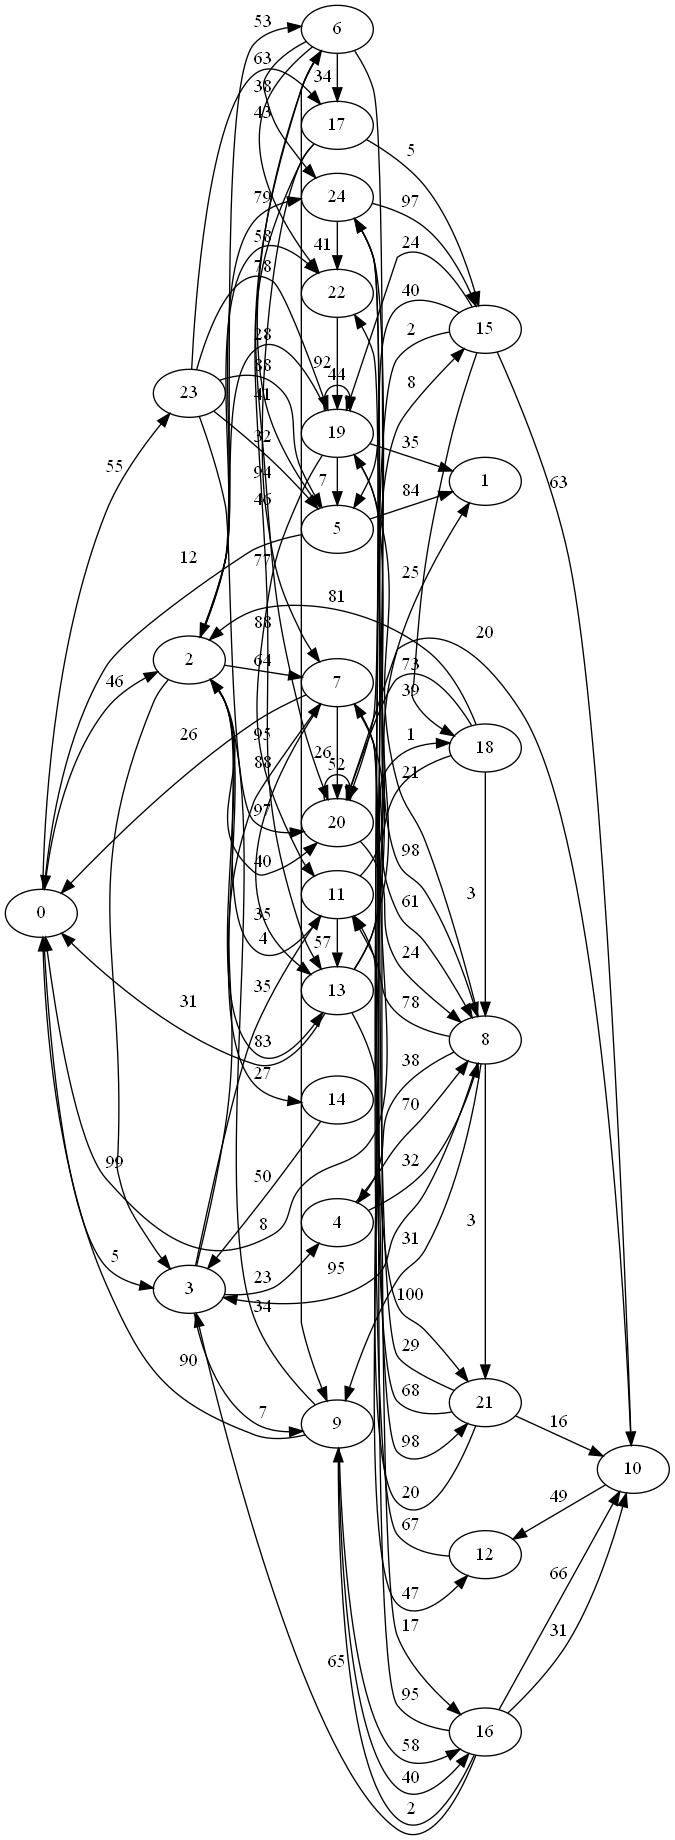
\includegraphics[scale=0.4]{pp0.png}
\end{center}
\subsection{Depth first search and edge classification}
There are two functions that perform DFS for every unvisited node and classify the edges.
\subsubsection{vector runDFS(vector,int)}
\label{dfs}
This function is called first. It creates a few data structures for storing the start and end times of visiting a vertex, order of nodes reached during the search, parents and children in the DFS tree. Then for every vertex it checks if the vertex is unvisited, then it calls the below function for that vertex.
\subsubsection{vector traverseDFS(int,vector)}
This function stores all the information in the above mentioned data structures. For detecting the edge types, the logic is as follows-\newline For every edge-
\begin{itemize}
	\item \textbf{If the destination node is unvisited}\newline
	This edge points to a visited node from an unvisited node. So, it will be a tree edge, always.
	\item \textbf{Else}
	\begin{itemize}
		\item \textbf{If end time of the destination node is not yet calculated}\newline
		This edge points from a visited node to a visited but unfinished node, so it will be a back edge.
		\item \textbf{Else if start time of source node is smaller than that of the destination node}\newline
		This edge points to a node which is visited later from a node which is visited earlier. But, since it is not a tree edge, so, it will be a forward edge.
		\item \textbf{Else}\newline
		For all other cases, the edge will be a cross edge.
	\end{itemize}
\end{itemize}
\subsubsection{Example}
The following is a graph indicating all the start and end times along with the edge classifications.
\begin{center}
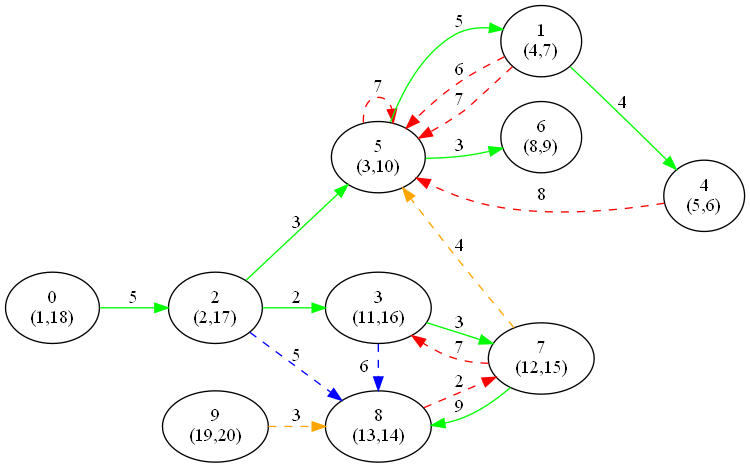
\includegraphics[scale=0.4]{pp1.png}
\end{center}
\textbf{Solid green edges:} - Tree edges\newline
\textbf{Dashed red edges:} - Back edges\newline
\textbf{Dashed blue edges:} - Forward edges\newline
\textbf{Dashed yellow edges:} - Cross edges\newline
Time complexity is $O(V+E)$.

\subsection{Strongly Connected Components using Tarjan's Algorithm}
There are two functions that implement \textbf{Tarjan's Algorithm} for finding the strongly connected components.
\subsubsection{vector runTarjan(vector)}
\label{tarjan}
This function is called first. It creates a few data structures for storing discovery and low times of all the vertices. Then for each vertex whose discovery time is 0 i.e. which is not yet discovered, it calls the DFS function specific for Tarjan's algorithm i.e. the below function for that vertex.
\subsubsection{vector runDFSForTarjan(int,vector)}
This function stores all the informations in the above data structures and follows Tarjan's algorithm to return the list of strongly connected components. In the algorithm, the key step is to update the low value to be the minimum of low of source and destination vertices if the edge is a tree edge and the minimum of low of source vertex and discovery of destination vertex if the edge is a back edge. We use a stack to keep track of the order of vertices visited. Then we keep popping from the stack till we reach the current vertex. All the popped vertices belong to a single strongly connected component.
\subsubsection{Example}
The following is a graph indicating all the strongly connected components.
\begin{center}
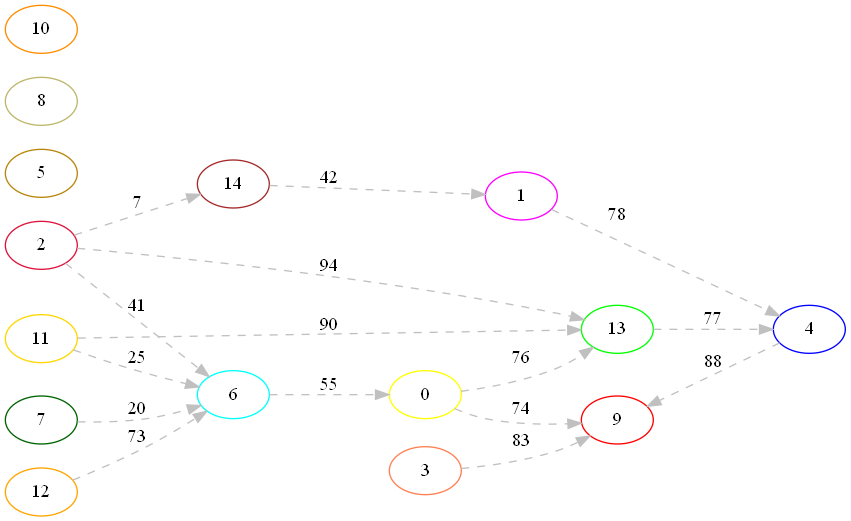
\includegraphics[scale=0.4]{pp2.png}
\end{center}
Each different colour represents a different strongly connected component. That means all the vertices and edges belonging to a single strongly connected component have one colour and the colour is unique. The dashed grey edges represent the edges connecting two strongly connected components.\newline
Time complexity is $O(V+E)$.

\subsection{Build a minimal graph by removing the redundant edges}
There are two functions that find the minimal graph of a given graph. Minimal graph is a graph obtained from the original graph which has same component graph and same strongly connected components but minimum possible edges. That means we reduce the edges and not the reachability. For performing these operations, first we run a DFS using \nameref{dfs} to get the edge classifications and the parents and children. Then we use \nameref{tarjan} to find all the strongly connected components. Then we use \nameref{dag} to get the DAG of the graph. All these information will be used while adding the set of minimal edges to the new graph.\newline
We divide the further process into two steps.
\begin{enumerate}
	\item Adding the edges falling within the strongly connected components.
	\item Adding the edges connecting two different strongly connected components.
\end{enumerate}
\subsubsection{void addEdgesWithinSCC(Graph,vector,vector)}
When we add the edges inside a strongly connected component, we follow a few steps.\newline
\textbf{Step-1: Add all the tree edges}\newline
This step makes the further steps easier.\newline
\textbf{Step-2: Ignore all the forward edges}\newline
Since we can reach from the same source to the same destination by using the tree edges, we do not need any forward edge.\newline
\textbf{Step-3: Assumptions for cross edges}\newline
If there are multiple cross edges from a single source vertex to different destinations, we consider only one cross edge that reaches the destination with lowest starting time. This is a greedy choice, since by doing this we can reach a larger set of vertices using the cross edge followed by some tree edges.\newline
\textbf{Step-4: Assumptions for back edges}\newline
Addition of back edges is the lengthiest step. Because, till now we have reachability from the root of the DFS tree to the leaves. The remaining step is to add the edges which will help us reaching back the root from the leaves. So, for each leaf node we have to find a path back to the root of the strongly connected component. Hence, we find all the nodes who do NOT have any children or their children belong to a different strongly connected component and add such nodes to a queue. Till this queue becomes empty we dequeue them one by one and add them to another queue.\newline
So for each leaf node, till the second queue becomes empty we dequeue them one by one and for all the backedges starting from that vertex, we choose the edge having a larger reachability i.e. we choose the edge whose destination is having the lowest start time. Then we add it to the minimal graph only if it the nodes on the path are not subset of any other backedge or vice versa. This checking is done by \nameref{reachCheck}. Then we enqueue the destination to the second queue. If the vertex does not have any backedge then we add its children to the queue. We repeat this process till we reach the root of the component.

\subsubsection{int * isSubset(vector,int,int,int)}
\label{reachCheck}
This function checks whether the current backedge is a subset of any previously added back edge or vice versa. The backedge which is a subset will be removed from the final graph.

\subsubsection{void addEdgesInterSCC(Graph,Graph,vector,vector)} 
For this, if there are multiple edges from one strongly connected component to another, then we consider only one out of them.

\subsubsection{Example}
The following is the minimal graph of the above considered graph.
\begin{center}
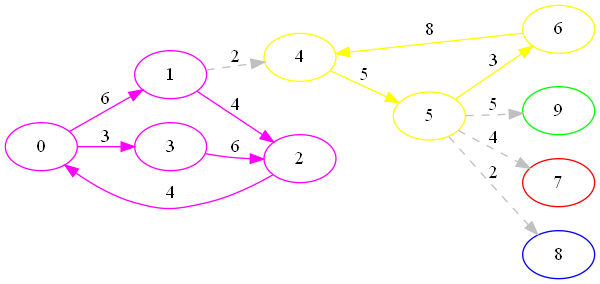
\includegraphics[scale=0.5]{pp6.png}
\end{center}
We can see all the strongly connected components are intact and the edges are minimal. Any further removal will destroy the connectivity of the graph.

\subsection{Check if the graph is semi connected or not}
There are three functions that help in checking whether the graph is semi connected or not. First we find all the strongly connected components using \nameref{tarjan}. Then we use those components to build a Directed Acyclic Graph by calling below function.
\subsubsection{void buildDAG(vector,Graph)}
\label{dag}
The DAG for the above graph will look like-
\begin{center}
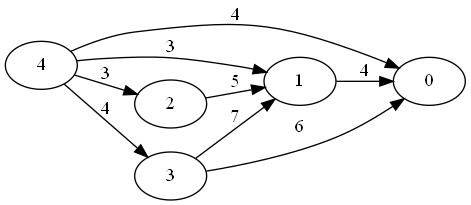
\includegraphics[scale=0.5]{pp3.png}
\end{center}
It actually takes one strongly connected component as one vertex. So we are not left with any more cycles in the new graph. Then we run Topological Sort on this graph by calling the below function.
\subsubsection{int * runTopologicalSort()}
This function implements topological sort and returns the sorted vertices. Then we call the below function.
\subsubsection{bool checkSemiConnected(int *)}
This function checks if each adjacent verteices in the topological order has a path either $u-->v$ or $v-->u$ or both.\newline
Since, we can see this is not the case for the above DAG, so our example is not semi connected.
\subsubsection{Example}
The following is a graph which is semi connected. The DAG is also given after it.
\begin{center}
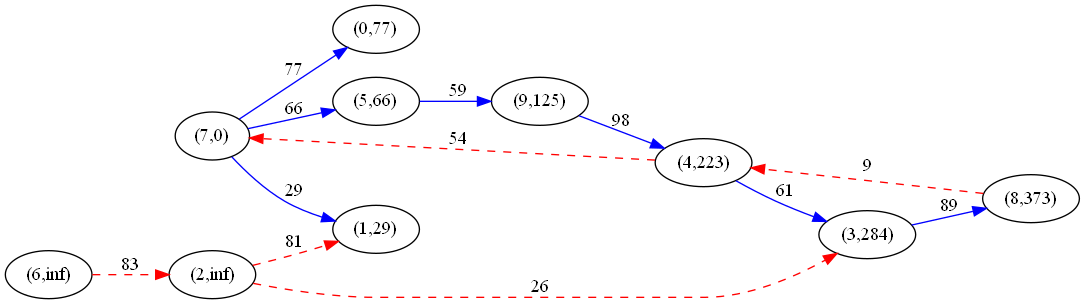
\includegraphics[scale=0.4]{pp7.png}
\includegraphics[scale=0.5]{pp8.png}
\end{center}
Time complexity is $O(V+E)$ for Tarjan's algorithm, $O(V+E)$ for building a DAG, $O(V+E)$ for Topological Sort and $O(V)$ for checking semiconnection property. In total it is $O(4(V+E))$ i.e. $O(V+E)$.

\subsection{Find shortest paths using Dijkstra's Algorithm}
There are two functions that implement \textbf{Dijkstra's Algorithm} for finding the shortes path distance from a particular source vertex to all other vertices.
\subsubsection{int * runDijkstra(int)}
This function is called first. It creates a few data structures for storing the path costs and the parent nodes. A min heap is implemented from scratch to keep track of the minimum cost vertices. This function extracts the root of the min heap $V-1$ times and calls the below function for each edge starting from that particular vertex.
\subsubsection{int * relaxEdge(Heap,int *,int,int,int)}
This function relaxes an edge. If the cost of the destination vertex is updated during relaxation, the cost is updated and decrease key operation is done on the heap.
\subsubsection{Example}
The following is a graph indicating the edges which participate in shortes path.
\begin{center}
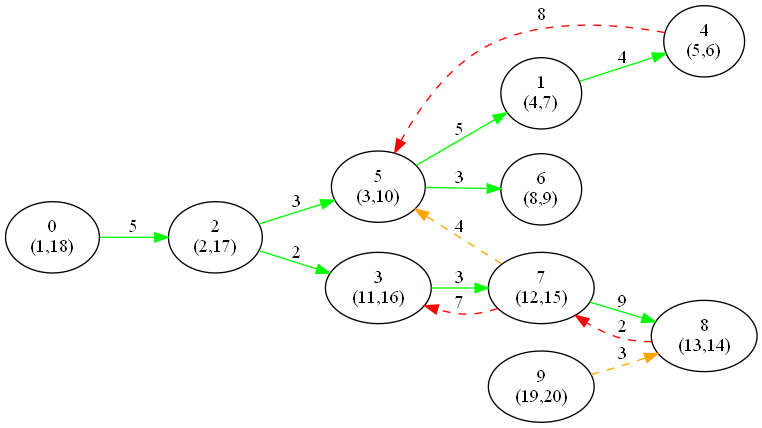
\includegraphics[scale=0.4]{pp5.png}
\end{center}
Source vertex is $12$. Solid blue edges participate in shortest path while the dashed red edges do not.\newline
Time complexity is $O(V+E\log V)$ since a min heap is implemented from scratch.

\section{Flow of Execution}
\subsection{User Prompt}
\begin{center}
\includegraphics[scale=0.55]{cmd1.png}
\end{center}
\begin{center}
\includegraphics[scale=0.55]{cmd2.png}
\end{center}
\begin{center}
\includegraphics[scale=0.55]{cmd3.png}
\end{center}
\begin{center}
\includegraphics[scale=0.55]{cmd4.png}
\end{center}
\begin{center}
\includegraphics[scale=0.55]{cmd5.png}
\end{center}

\subsection{Example Testcase}
\subsubsection{For creating a graph}
23 34\newline
0 1 10\newline
0 2 3\newline
1 2 1\newline
1 3 2\newline
2 1 4\newline
2 3 8\newline
2 4 2\newline
3 4 7\newline
4 3 9\newline
5 6 4\newline
6 7 8\newline
7 5 3\newline
6 8 5\newline
6 9 7\newline
6 11 3\newline
8 10 5\newline
9 10 8\newline
12 13 6\newline
12 15 3\newline
13 14 4\newline
13 16 2\newline
14 12 4\newline
14 18 3\newline
15 14 6\newline
16 17 5\newline
16 18 1\newline
17 18 3\newline
17 19 4\newline
17 20 2\newline
17 21 5\newline
18 16 8\newline
19 21 3\newline
20 21 4\newline
21 20 7\newline\newline
It means there are 23 vertices and 34 edges. The rest of the rows are in the format \textbf{source destination weight}.
\subsubsection{Modifying a graph in bulk}
1 2 4 5\newline
1 4 6 7\newline
2 4 5\newline\newline
It means\newline
1 2 4 5 (Add an edge from 2 to 4 with weight 5)\newline
1 4 6 7 (Add an edge from 4 to 6 with weight 7)\newline
2 4 5 7 (Remove the edge from 4 to 5 with weight 7)

\subsection{Instructions to execute the code}
\begin{enumerate}
	\item If you're using Dev C++, Follow the steps to support $unordered\_map$. Go to tools--compiler option--general tab--tick mark option (add the following commands when calling compiler)--add -std=c++11 there. Then build and execute the project.
	\item In linux or GNU windows compiler, open the terminal or command prompt and type "g++ GraphImpl.cpp" and hit enter.
	\item Then for linux type "./a.out". For windows type "a.exe" or "GraphImpl.exe" (One of them should work). Hit enter.
	\item You can also write "./GraphImpl" and hit enter to execute the makefile which is provided.
	\item Now the prompt will be displayed. Enter 0 or 1 for windows or linux respectively.
	\item Give a name for all the files which are going to be generated during execution.
	\item Write a .txt file according to the given format and enter the file name there.
	\item The entire execution process can be visualized in $<user\_given\_name>Output.txt$.
	\item After printing a graph, you can view the images in the same directory. The respective file names are written in the output file.
	\item You can give multiple .txt files one after another. For example- in the first run, you can create a very dense graph, find the minimal graph and replace it with the original one, remove a few edges and then proceed for shortest paths or strongly connected components. Later you can create a new graph and do the same processing on it. All the images will be stored simultaneously.
	\item You can run the batch file or shell script to manually generate the images.
	\item Avoid giving percentage more than $50$. It is going to create a mess and you won't be able to visualize it. Moreover, there is a huge possibility of having only a single strongly connected component.
	\item There will always be an option to go back to the main menu so that you can either generate all the images for the graphviz files written till now or quit.
\end{enumerate}

\section{Testing}
\subsection{Minimal Graph Example - 1}
\begin{center}
\includegraphics[scale=0.3]{pp9.png}
\end{center}
\begin{center}
\includegraphics[scale=0.3]{pp10.png}
\end{center}
\subsection{Minimal Graph Example - 2}
\begin{center}
\includegraphics[scale=0.3]{pp11.png}
\end{center}
\begin{center}
\includegraphics[scale=0.3]{pp12.png}
\end{center}
\subsection{Minimal Graph Example - 3}
\begin{center}
\includegraphics[scale=0.3]{pp13.png}
\end{center}
\begin{center}
\includegraphics[scale=0.3]{pp14.png}
\end{center}
\subsection{Minimal Graph Example - 4}
\begin{center}
\includegraphics[scale=0.3]{pp15.png}
\end{center}
\begin{center}
\includegraphics[scale=0.3]{pp16.png}
\end{center}
\subsection{Minimal Graph Example - 5}
\begin{center}
\includegraphics[scale=0.2]{pp17.png}
\end{center}
\begin{center}
\includegraphics[scale=0.15]{pp18.png}
\end{center}
\subsection{Dijkstra's Algorithm : Source = 14}
\begin{center}
\includegraphics[scale=0.2]{pp19.png}
\end{center}

\end{document}